\subsection{Architecture}

This section aims to give a broad view of the components and how each one work together to satisfy satisfy the need of our prototype. A more detailed explanation for each component will be discussed in section \ref{sssec:technologies}. 

\begin{figure}[t]%evtl:[t] [!htbp]
\centering
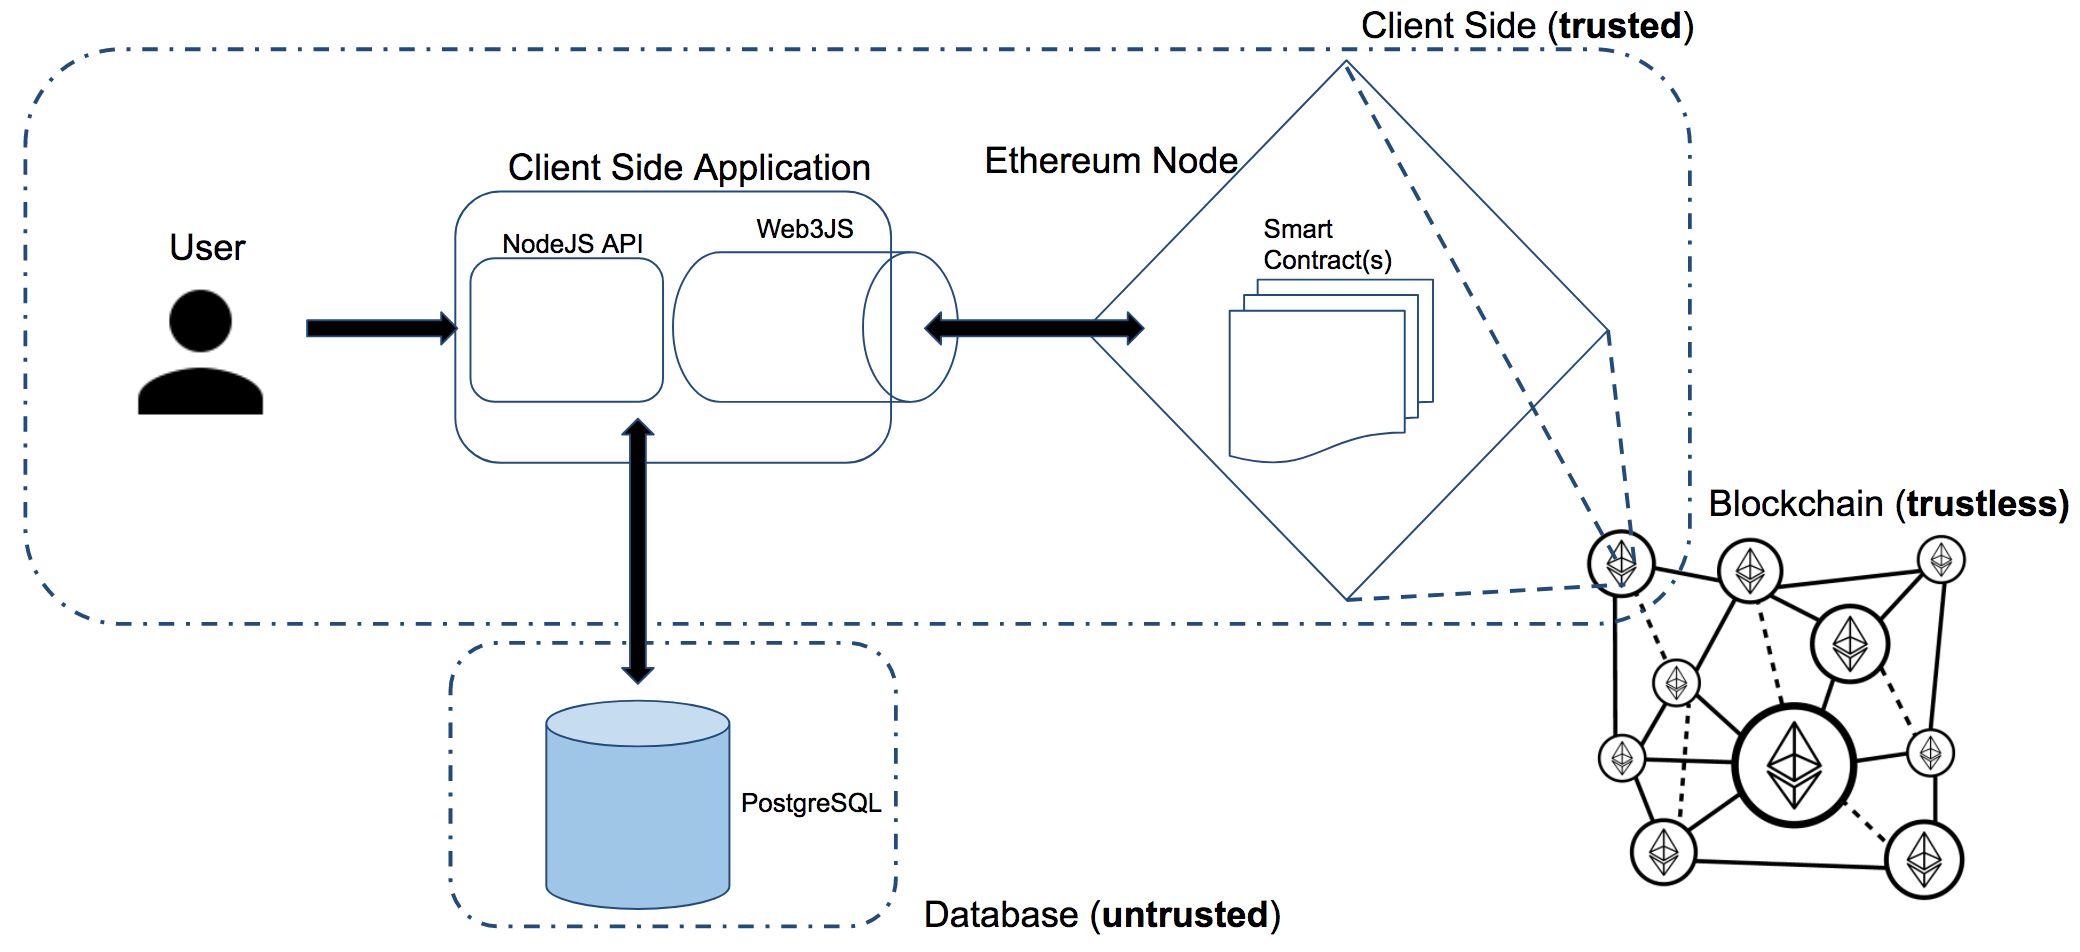
\includegraphics[width=1.0\textwidth]{images/architecture.png}
\caption{\label{fig:architecture}The architecture of the off-chaining approach.}
\end{figure}

As seen in Figure \ref{fig:architecture}, we have divided our architecture into three sides: 
\begin{itemize}
\item Client side
\item Database
\item Blockchain environment
\end{itemize}

\paragraph{Client Side}
The client side consists of the client side application, and the Ethereum node. The client side application is the biggest component as it bridges the database and the Smart Contract in the Ethereum Node. Currently, we still put trusts into the client side to a certain extent. The extent of trust varies depending on the use case, but nevertheless, a certain level of trust has to exist. For example, upon insertion of new data, before any data goes into the Smart Contract to be processed, we trust that the client side application will not alter the values. This assumption also acts as a temporary solution to the gas cost problem. Hence, it allows us to perform the proof-of-concepts in our use cases. See section \ref{sssec:use_cases} to learn more about how our use cases handle this problem.


\paragraph{Blockchain Environment}
The Blockchain environment is the decentralized network where the Smart Contract and its local data going to ultimately live in. The Blockchain decentralized network is trustless. But what it truly means is that the trust is distributed to all ledgers in the network. It also means that we do not enforce an external force to make sure that the Smart Contract and its local data are accurate and consistent (integrity). The environment itself ensures the integrity of the data. 

\paragraph{Database}
The database however, is not trusted. Though in our approach we use the database to store data that is going to be used again in the Smart Contract, we cannot trust the database. The database is prone to internal attacks that can affect the integrity of the data. But at the same time, a database allows us to store large amount of data, and it can be easily integrated with other applications or systems, highly suitable for an off-chaining approach. Hence our approach includes leveraging data integrity check mechanisms when using off-chained data in Smart Contract.

\paragraph{Transportation}
We have not only made the assumption that our client side is trusted, but also the the transportation layer is secured. Prior to the assumption, we have thought of attacks such as the man-in-the-middle attack, and how determinantal this attack is when we want to save raw data to the database, or when communicating with the Smart Contract. For example, it can be that the hashes created in the client side application are altered upon sending them to the Smart Contract during the initial step. The first step of the approach includes the client side application hashing the raw data and sending the hashes to the Smart Contract to be stored, mapping the off-chained data to their hashes. Hence, if an attack changes a hash to a different data’s hash, then someone may be able to pass the integrity check by using that altered hash’s raw data value. 

These assumptions are made due to the gas-cost problem ...////////////see reference somewhere?.... In the future, we would want to abandon these assumptions and solve these problems accordingly. See section \ref{sec:future_work} to learn more on the potential solutions.
